\documentclass{article}

\usepackage[utf8]{inputenc} % allow utf-8 input
\usepackage[T1]{fontenc}    % use 8-bit T1 fonts
\usepackage{hyperref}       % hyperlinks
\usepackage{url}            % simple URL typesetting
\usepackage{booktabs}       % professional-quality tables
\usepackage{amsfonts}       % blackboard math symbols
\usepackage{nicefrac}       % compact symbols for 1/2, etc.
\usepackage{microtype}      % microtypography
\usepackage{graphicx}
\usepackage{cite}
\usepackage{xcolor}
\usepackage{listings}
\lstset{basicstyle=\ttfamily,
    showstringspaces=false,
    commentstyle=\color{red},
    keywordstyle=\color{blue}
}


\title{DeepSV: a deep learning based variant scorer}

\author{
  Félix Raimundo\\
  Department of Computer Science\\
  École Polytechnique\\
  Palaiseau, France\\
  \texttt{felix.raimundo@inria.fr}
  %% examples of more authors
  %% \And
  %% Coauthor \\
  %% Affiliation \\
  %% Address \\
  %% \texttt{email} \\
  %% \AND
  %% Coauthor \\
  %% Affiliation \\
  %% Address \\
  %% \texttt{email} \\
  %% \And
  %% Coauthor \\
  %% Affiliation \\
  %% Address \\
  %% \texttt{email} \\
  %% \And
  %% Coauthor \\
  %% Affiliation \\
  %% Address \\
  %% \texttt{email} \\
}

\begin{document}

\maketitle

\begin{abstract}
  In this paper, we present DeepSV, a deep learning based method for scoring the likelihood that a set of adherent read pairs are caused by a structural variant, by opposition to mapping or sequencing errors.
  
  We identified a region of fixed size that contains enough signal to make classification
  with deep learning methods, and thus allowing us to move away from the previous methods
  based on linear classifiers applied on few hand-crafted features.
\end{abstract}

\section{Definitions}

In this papers we will be using the sequencing terms as defined in \cite{li_sequence_2009}, whose most
relevant ones are copied here.

\paragraph{Segment} A contiguous sequence or subsequence.
\paragraph{Read} A raw sequence of DNA that comes off a sequencing machine.
\paragraph{Coverage} Number of reads mapped at a specific location in the reference genome.
\paragraph{Read Pair} Long sequence of DNA of which the sequencing machine reads the two extremities. Each of the two extremities are reads and are associated a direction and are separated by a distance called insert size.

Note: For the duration of this paper, we will assume that the two reads of a read pair are both directed to the center, i.e. the first read is directed from left to right, called forward, and the second right to left, called backward.

\section{Properties of the data}

In this paper we will be making the following two assumptions:

\paragraph{Property 1} The distance between two reads of a read pair, called insert size, follows a normal distribution.
\paragraph{Property 2} The length of reads, called read size, follows a normal distribution.

Note: there are no guarantees that they are true, nevertheless they are a good approximation of reality and are used in most other variant callers (see \cite{ rausch_delly:_2012}, \cite{ye_pindel:_2009}, \cite{chen_manta:_2016}, \cite{handsaker_large_2015}, \cite{chen_breakdancer:_2009}).

Note: The distance between two reads of a pair generated from a target genome can be different once the two reads are mapped on a reference genome, the analysis of that phenomenon is the basis of our study.

\paragraph{Hypothesis 1}: During the rest of this document we will assume that the insert size and read size are constant when the reads are generated, indeed the two distribution have a low standard deviation, this approximation is thus sensible.
All the future claims stay valid with this approximation, but would make the text much less readable.

Section \emph{Dealing with reality} will describe how we deal with real data, where these assumptions are not correct.

\paragraph{Property 3} Because of properties 1 and 2, and hypothesis 1, it follows that the second pair of a read pair is fully contained within $[insert\_size, insert\_size + read\_size]$ of the end of the first one in the genome from which the reads are extracted.

\subsection{Structural Variants}

\paragraph{Variant} We call variant, a difference between the genome of the person being sequenced and the reference genome, they are the cause of the genetic diversity in the population.

Some variants are called \emph{structural variants}, because they are considered so large that they come from a structural difference. The limit between regular variant and structural variant does not have a proper definition, but they are usually considered to be changes affecting more than 50bp.

Structural variants are separated in two categories:
\begin{itemize}
    \item Balanced rearrangements: which do not affect the total number of nucleotides in the genome.
    \item Imbalanced rearrangements: which affect the total number of nucleotides in the genome, also called Copy Number Variation (CNV).
\end{itemize}

The CNVs are themselves divided in three categories:
\begin{itemize}
    \item Deletions: where a large portion of the genome is deleted relative to the reference.
    \item Tandem duplication: where a large portion of the genome is duplicated, potentially multiple times; the duplicates are directly next to each other.
    \item Interspersed duplication: where a large portion of the genome is duplicated, potentially multiple times;
    the duplicates are separated by segments of DNA.
\end{itemize}

Likewise the balanced rearrangements are divided in two categories:
\begin{itemize}
    \item Translocation: where a large portion of DNA is moved to another location in the genome (potentially on another chromosome).
    \item Inversion: where a large portion of DNA has the order of its nucleotides reversed.
\end{itemize}

In our study we will only work on deletions, tandem duplications, and inversions. We however believe that our method could be extended to work on the other types of variants (see \emph{Future Work}).

\paragraph{Breakpoint} We call breakpoints the locations where structural rearrangements happen in the genome , there are:
\begin{itemize}
    \item 1 in the case of deletions.
    \item $n$ for tandem duplications with $n$ duplicates.
    \item $n$ for interspersed duplications with $n$ duplicates.
    \item 2 for inversions
    \item 2 for translocations.
\end{itemize}

\subsection{Methods of detection}

The current state of the art algorithms for finding structural variants are based on a mixture of the four following methods (see \cite{lin_making_2015} or \cite{sudmant_integrated_2015} for a deeper review):

\begin{itemize}
	\item Assembly based (AS), does \emph{de novo} assembly on regions suspected to contain an SV. They are rarely used as: assembly is computationally expensive, and not always possible in regions with repetitive sequences.
	\item Read count (RC), observes the distribution of coverage in the genome. It can only detect CNVs as reads in translocations and inverted regions are properly mapped. Furthermore reads are not generated uniformly in the genome from which the reads come, it is thus not an optimal method alone.
	\item Split reads (SR), uses reads that fall on the breakpoint. Those reads are unmapped, as part of them is in the rearrangement. These reads are split so that they can be mapped properly. As the split reads are smaller than regular reads they cannot always be mapped unambiguously.
	\item Paired reads (PR), uses pairs of mapped reads that have an insert size far away from the mean insert size, or who do not have the expected orientation. This method is often used to identify regions that contain SV and followed by a finer analysis of the candidate.
\end{itemize}

In the case of DeepSV we use paired reads to identify regions of interest and use a pattern recognition model on the selected regions to decide whether they contain an SV.
We expect our model to use RC and PR methods for predictions. AS and SR methods can be used to locate the breakpoints with higher precision once the prediction is made.

The next sections will explain what patterns we expect to find in these regions.

\subsection{Anomalous paired reads}

Anomalous read pairs (ARP) are read pairs that do not have the normal orientation or distance.

\paragraph{Property 4}  Assuming no errors in the reads or mapping, ARPs contain a breakpoint between their two reads.

Indeed, if one read was on the breakpoint, it could not be mapped as a part of it would be on a large rearrangement.

Respectively, if both reads were the same side of a  breakpoint, they would be mapped normally and would
thus not be caught as anomalous.

\paragraph{Property 5} Because of properties 3 and 4 we can conclude that all reads in ARPs will be at most $read\_size + insert\_size$ away from the breakpoint in the genome that generated the reads.

\subsubsection{Deletion}

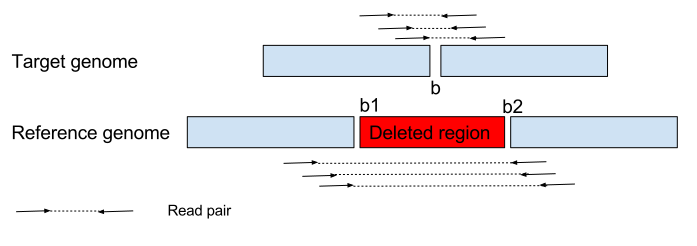
\includegraphics[width=\textwidth]{DeletionReadPairs}

In the case of deletions there is a single breakpoint $b$, the deleted region is $[b1, b2]$.

Assuming no errors in the reads or mapping:
\begin{itemize}
    \item reads to the left of b are mapped left of b1 in the reference genome.
    \item reads to the right of b are mapped to the right of b2 in the reference genome.
    \item no reads should be mapped in $[b1, b2]$.
\end{itemize}

We can conclude that given a set of ARPs supporting a deletion, b1 will be contained within $insert\_size + read\_size$ of the leftmost read, and b2 will be contained within $insert\_size + read\_size$ of the rightmost read.

Furthermore, the previous observations, allows us to tell that all ARPs will be contained in that region. If we also add some content from the deleted section we can observe the coverage there and compare it to the coverage outside the deleted region.

We have thus constructed two intervals containing all the ARPs and RC information, these two intervals' sizes are only dependant on the insert size and read size, not the size of the deletion. 

\subsubsection{Inversion} 

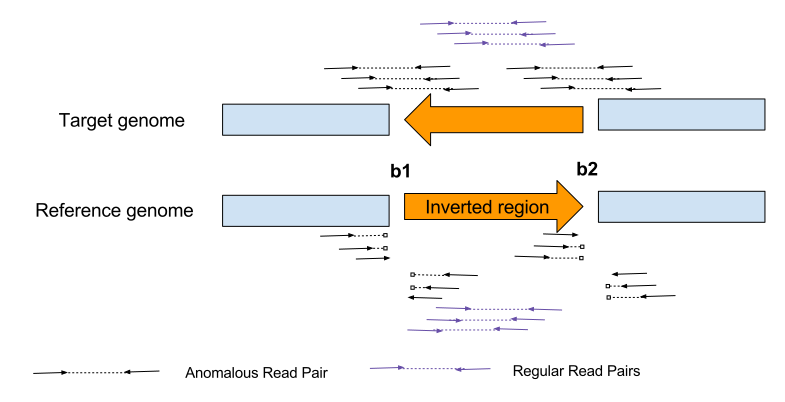
\includegraphics[width=\textwidth]{InversionReadPairs}

Here ARPs are pairs where one read is in the inversed region and the other
is in the regular one (i.e. either one read left of b1 or one read right of b2). Indeed reads
between b1 and b2 will be mapped properly (because BWA is not sensitive to the order of the reads).

Reads in the inversed region will be mapped in the wrong direction, and farther away
than expected (as the region is inversed they will be moved closer to the other breakpoint).

We can see that if one read is left of b1, the other one will be mapped close to
b2 inside the inversed region and in the wrong direction, and that if one read is to the right
of b2, the other one will be mapped close to b1 in the inversed region and in the wrong direction
too.

We can also see by using properties 1 and 2, that reads outside the inversed region will be at most
\verb|insert_size + read_size| away from the breakpoints and that the same is true for reads inside
the inversed region.

\paragraph{Lemma 4} ARPs supporting an inversion will be distributed around the two
breakpoints within \verb|2*(insert_size + read_size)|.

\paragraph{Lemma 3} Respectively, should we have a group of ARPs supporting the same inversion we can say with a known confidence interval, that most ARPs around the left breakpoint will be contained within \verb|2 * (insert_size + read_size)| of the beginning of the leftmost supporting read. The same is trivially true for the right breakpoint.

\subsubsection{Tandem Duplication}

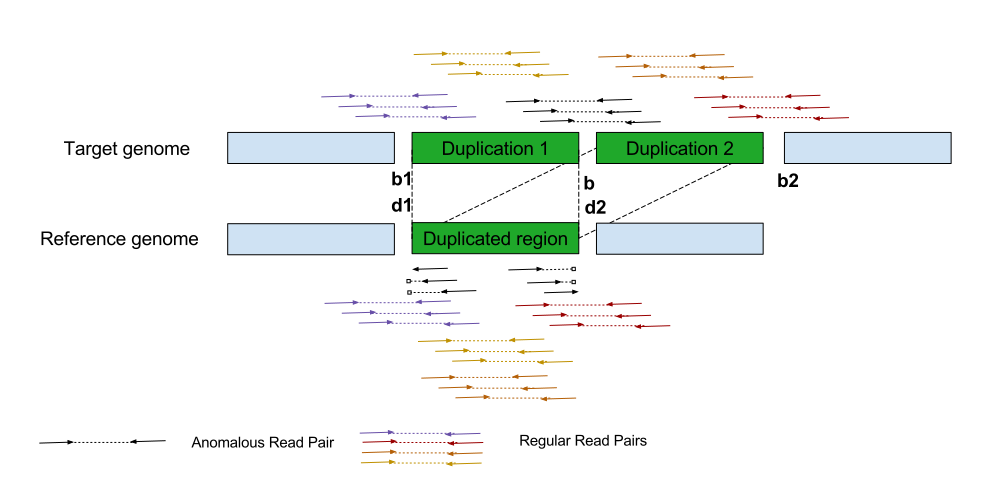
\includegraphics[width=\textwidth]{DuplicationReadPairs}

Here ARPs, are pairs that have one read on each side of breakpoint b, indeed
read pairs fully contained between b1 and b or b and b2, will be mapped properly on the
duplicated region.

\paragraph{Lemma 6} ARPs are aligned in the wrong direction (\verb|<- ->| instead of \verb|-> <-| for example), and inside the duplicated region, one within \verb|insert_size + read_size| to the right of d1, the other within \verb|insert_size + read_size| left of d2.
The read count in the duplicated region will be about the double of outside the duplicated region.

\paragraph{Lemma 7} It follows that should a region be duplicated more than once, the ARPs will be distributed the same way as with tandem duplication (except for higher read count and more ARPs).

\subsection{Conclusion}

\paragraph{Theorem 1} Putting all the lemmas together we can conclude that given a set of structural variants, there are two windows of size \verb|2 * (insert_size + read_size)| each, centered on the two breakpoints in the reference genome that contains most of the ARPs that will support it.

\paragraph{Theorem 2} Given a type of variant and a set of supporting ARPs, we can construct two windows of size \verb|2 * (insert_size + read_size)| that will contain the breakpoints in the reference genome.

\paragraph{Note} For tandem CNVs (and deletions) windows of size \verb|insert_size + read_size| would have sufficed to contain all the ARPs, however they would not have contained reads outside of the duplicated area (inside the deleted area), which would make us lose the RC information.
Taking larger windows also allows us to have a single window size for all our variants, and thus using the same model for all the variants.

\paragraph{Note} All the window sizes given here assumed that the reads and inserts were of the same size, when we know that they are variable, adding a few standards deviations will allow us to catch the read pairs with higher insert size or read size. \cite{pham_efficient_2018}

\section{Dealing with real data}

As said before, the empirical insert size does not follow a normal distribution. We can see that it is skewed towards lower values. However, we can see that the distribution is well centered on its mean: 400 bp.

\includegraphics[width=\textwidth]{insert_size_histogram}

\begin{lstlisting}[language=bash,caption={Picard command}]
#!/bin/bash
java -jar picard.jar CollectInsertSizeMetrics \
    I=input.bam \
    O=insert_size_metrics.txt \
    H=insert_size_histogram.pdf \
    M=0.5
\end{lstlisting}

We are aware of two reasons that could cause such a skew:
\begin{itemize}
    \item Mobile element insertions of ALUs.
    \item Poor mapping in ambiguous regions.
\end{itemize}

Picard tells us that a width of 165 centered on the median, 386bp, will catch 95\% of the reads,
which will be considered a sufficient approximation. In consequence when building our window we will
consider an insert size of 467bp.


\section*{References}

\bibliography{deepSVbib.bib}{}
\bibliographystyle{unsrt}

\end{document}